%{{{ Spam
\documentclass[a4paper,12pt]{article}

%use danish hyphenation and titles
%handle utf8-characters
\usepackage[danish]{babel}
\usepackage[utf8]{inputenc}
\usepackage[T1]{fontenc}

%for images
\usepackage[pdftex]{graphicx}

%allow nested figures
\usepackage{subfigure}

%control line spacing
\usepackage{setspace}
%\singlespacing
\onehalfspacing
%\doublespacing

%set margins
%\usepackage[margin=0.75in]{geometry}

%allows margin-notes
%good for work in progress papers
%\usepackage{marginnote}

%allows pretty quoting using ``'' or `'
\usepackage{upquote}

%two definitions of the color grey
\usepackage{color}
\definecolor{listinggray}{gray}{0.9}
%\definecolor{lbcolor}{rgb}{0.9,0.9,0.9}


% References
\usepackage{hyperref}

%allows pretty source code
\usepackage{listings}
\lstset{
  language=,
  literate=
    {æ}{{\ae}}1
    {ø}{{\o}}1
    {å}{{\aa}}1
    {Æ}{{\AE}}1
    {Ø}{{\O}}1
    {Å}{{\AA}}1,
  backgroundcolor=\color{listinggray},
  tabsize=3,
  rulecolor=,
  basicstyle=\scriptsize,
  upquote=true,
  aboveskip={1.5\baselineskip},
  columns=fixed,
  showstringspaces=false,
  extendedchars=true,
  breaklines=true,
  prebreak =\raisebox{0ex}[0ex][0ex]{\ensuremath{\hookleftarrow}},
  frame=single,
  showtabs=false,
  showspaces=false,
  showstringspaces=false,
  identifierstyle=\ttfamily,
  keywordstyle=\color[rgb]{0,0,1},
  commentstyle=\color[rgb]{0.133,0.545,0.133},
  stringstyle=\color[rgb]{0.627,0.126,0.941},
}
%captions on listings
\usepackage[center,font=small,labelfont=bf,textfont=it]{caption}

%allows fancy enumeration
\usepackage{enumerate}

%allows use of the BibTex for the bibliography
\usepackage[numbers]{natbib}

%make references and URLs in the pdf to clickable links
\usepackage{hyperref}

%removes the numbers from sections
\setcounter{secnumdepth}{0}

%proper header formatting
\usepackage{fancyhdr}
\pagestyle{fancy}
\lhead[]{} %clear standard settings
\chead[]{} %clear standard settings
\rhead[]{\rightmark} %current section
\lfoot[]{} %clear standard settings
\cfoot[]{\thepage} %current page number 
\rfoot[]{} %clear standard settingsF

\usepackage{hyperref} % The package for links. This is also used for the ToC links.
%}}}
\title{Heartbeat protokollen
\\
Bachelorprojekt 2015}
\author{Erik Allin - smt504 \\ Dennis Olesen - cwb579}
\date{??. juni 2015}

%Centreret sidehoved
\chead{Erik Allin - smt504 \& Dennis Olesen - cwb579}

\begin{document}
\maketitle
\newpage
%\renewcommand*\contentsname{Table of Contents}
%\tableofcontents
%\section*{Forside-lel}
%\newpage
%\clearpage


\section*{Beskrivelse af problemet}
\subsection*{Motivation}
I forbindelse med udvikling af et distribueret system vil man være afhængig af, at kunne sikre sig konsistens samt høj tilgængelighed af det involverede system. Metoder til at opdage når en maskine fejler, samt derefter at foretage de nødvendige fejlprocedurer, vil altså være at finde i størstedelen af de distribuerede systemer.
Ved at konstruere et bibliotek, som gør det simpelt for brugeren at implementere disse metoder vil der både kunne spares udviklingstid for fremtidige projekter, der omhandler distribuerede systemer, og være et fælles produkt at kunne optimere og opdatere, fremfor at skulle tage hensyn til hvert enkelt nye system. Endvidere forventer vi, at man i forbindelse med dette samtidig kan opretholde en balancering af systemernes ressourcer, i forbindelse med de regelmæssige liveliness tjek. 
\\
Et sådant bibliotek vil herved kunne sikre fremtidige applikationer der bruger distribuerede systemer, en fælles og gennemtestet implementation til både load-balancing og liveliness tjek af deres systemer.

\subsection*{Redegørelse}
For at kunne lave et bibliotek til implementering af load-balancing via heartbeat protokollen, er vi nødt til, at forstå hvordan systemet skal hænge sammen.
I stil med Raft (se artikel) skal vi have en leder, der kan uddelegere opgaver, samt overvåge aktiviteten (liveness) for de resterende systemer. Dette kan lederen gøre ved regelmæssigt at sende heartbeats ud til alle de aktive følgere. I forbindelse med dette tjek af liveness, kan vi sende en værdi for belastningen med vores heartbeats, der sendes til følgerne. Dette tillader os, at lave en prioritering for hvilke følgere, der skal modtage næste opgave. 
Da vi er interesserede i, at systemet også skal have høj tilgængelighed er vi afhængige af at lederen ikke er en single-point-of-failure. Altså kort sagt må systemet ikke fejle når lederen fejler.
\\[5px]
Dette kan vi undgå ved, at have mulighed for at vælge en ny leder, når følgere i en længere periode ikke har modtaget heartbeats fra lederen. Dette gøres i stil med Rafts leadership-election. Heri anvendes der kandidater, som følgere kan skifte status til, hvis de mangler tilstrækkeligt med heartbeats fra lederen. Herudover gås der efter, at kandidaterne så vidt som muligt er up-to-date med loggen. Loggen er en metode, som vi bruger til at sikre os, at både leder og følgerne er enige om hvilken rækkefølge eventsne er blevet kørt i.
\\[5px]
Dette system vil altså afhænge af, at have fem del-funktionaliteter der tilsammen udgør systemet. Disse fem funktionaliteter kan ses som Discovery, hvor der oprettes forbindelse til følgere på netværket, samt liveness hvor der regelmæssigt tjekkes for, at følgere og leder er i live. Leader-election sikrer, at der hurtigt kan findes en ny leder, hvis den nuværende fejler. Logging sikrer sig, at der hele tiden er konsistens i systemet, så rækkefølgen af opgaver ikke går galt, når der vælges en ny leder. Til sidst er der load-balancing, som afhænger af at det resterende system fungerer, så det kan balancere belastningen af følgerne.

\section*{Analyse af problemet}
\subsection*{Discovery} 
For at skabe forbindelse til maskiner på et lokalt netværk, er man, som vi kom frem til i forrige afsnit, nødt til at benytte sig af en discovery protokol. Et sådant system kendes også som network Discovery services (INDSÆT REFERENCE TIL KAP. 19.2). Normen er her, at man opretter forbindelse til andre systemer i netværket, ved at broadcaste(multicaste) til sin lokale IP, og derved få beskeden ud til de resterende systemer. Dette virker som den oplagte måde, at gøre det på da der arbejdes på et lokalt netværk. Problematikken er i midlertidig om det er en directory server eller serverless model, der vil fungere bedst i forbindelse med resten af systemet. 
\\
Her kan man argumentere for, at en directory server ville give mening, da der i forvejen sendes regelmæssige broadcasts i forbindelse med heartbeat. Altså kunne man her bruge heartbeatet, som en forespørgelse til systemer, der ikke er forbundet med lederen endnu.
Directory server har dog det problem, at hvis den går ned, er der ikke længere styr på hvilke maskiner, der er i systemet. Dette er imidlertid en problematik som bør kunne løses med leader election, og logging, ved at man vedligeholder en replikeret log, som indeholder de aktive følgere, til alle medlemmer i systemet. Derved vil en ny leder have samme information, som den tidligere leder, og kan derved overtage jobbet uden at miste konsistens eller tilgængelighed. Ifølge DSCD, bruges der leasing til, at sikre sig, at maskinerne er aktive. Dette må kunne erstattes med heartbeats, da dette foretager samme tjek, altså ved feedback om et kald, el. en service går igennem.

\subsection*{Liveness} 
Liveness er langt hen ad vejen en af grundidéerne ved heartbeat. Derfor ligger det også naturligt, at liveness bliver tjekket via heartbeats, samt manglen heraf. Man kan definere et system til, at være i live, når det har forbindelse til lederen. Ved brug af leader election, som ses senere vil der altid være en ny leder, der kan erstatte en afgående, el. død leder (indenfor et rimelig interval). I praksis vil tjek for liveness ligge meget op ad det, der er omtalt i discovery-afsnittet. 
Dette grundet at heartbeats er måden hvorpå liveness tjekkes, og at listen over aktive, el. levende, systemer opbevares i en log, som bliver opdateret løbende igennem discovery-protokollen.

\subsection*{Leader election}
Leader election er en essentiel del af heartbeat systemet. Det sørger for at såfremt lederen, altså det system der modtager og videresender forespørgsler, skulle stoppe med at fungere, så vil der, under enighed mellem alle i systemet, blive valgt en ny leder.
\\
For at gøre dette, kan man, i stil med Raft, indføre tre stadier for systemerne:
\\ 
Følger, kandidat og leder.
\\
Disse fungerer ved, at ved at en følger kan blive kandidat, såfremt den ikke har modtaget beskeder fra lederen i en tidsbestemt periode. Når en følger bliver kandidat udsteder den et valg, og sender en forespørgsel om at blive valgt som en ny leder. Såfremt kandidaten får majoriteten af stemmerne, vil den blive valgt som den nye leder. Lederens rolle er at lytte på klienten som sender forespørgsler, og så sørge for at disse forespørgsler bliver sendt ud til de korrekte systemer, samt sikre sig konsistens i loggen. For at undgå at systemer der ikke er up-to-date kan være ledere, skal der indføres en logisk klokke til at holde styr på at alle systemer er lige langt. Dette sikrer at hvis en maskiner kommer ud af synkronisering vil den ikke forsøge at blive leder, samt at hvis en leder mister forbindelsen og der bliver valgt en ny leder, vil den når den kommer tilbage opdage at den ikke længere skal være leder, og derved skifte til følger. 


\subsection*{Logging}
For at systemet hele tiden kan holdes konsistent, må vi indføre en form for såkaldt logging. Logging sørger for, at alle medlemmer af systemet hele tiden kan holde styr på, om de er med i systemet. Hvis de f.eks. mister forbindelsen i en periode, og så kommer tilbage i systemet, så vil medlemmet højst sandsynligt være kommet bagud i forhold til resten af systemet, og derved skal medlemmet ikke f.eks. forsøge at blive kandidat, der vil kunne forsinke systemet (som også beskrevet i forrige afsnit). Loggingen laves via timestamps, så der hele tiden kan ses hvilket stadie de forskellige dele af systemet er nået til. Derudover holder loggingen også styr på rækkefølgen det hele skal foregå i, for derved at kunne se, hvis nogle opgaver ikke er blevet udført af de forskellige dele af systemet. Dette sikres ved, at loggen hele tiden holdes konsistent og hele tiden bliver replikeret ud til alle alle medlemmer af systemet. Derved sikres det også, at når en ny leder bliver valgt, så vil denne leder også have den have den log, som den forrige leder sad tilbage med, og derved går der ikke nogle opgaver tabt.


\subsection*{Load-balancing}
For at arbejdet i systemet hele tiden fordeles fair indføres begrebet load balancing. Dette sørger for, at der via heartbeats sendes en form for stress måling fra de forskellige systemer ud. Dette gør også, at hvis der er stærkere medlemmer i systemet, så kan disse få de mere krævende opgaver, og derved kan opgaverne blive fordelt, så det samlede arbejde bliver løst på den optimale tid.



\section*{Implementering}

\subsection*{Discovery / Liveness}
Discovery fungerer sådan i vores system, så at lederen i systemet broadcaster til den lokale broadcast IP-adresse, xxx.xxx.xx.255, i vores tilfælde dog 255.255.255.255 samt en vilkårlig, ikke-reserveret port. Herved kan der oprettes forbindelse til alle resterende IP-adresser på netværket, hvis forbindelsen altså lykkedes.
\\[5px]
Dette gøres via socket-biblioteket i Python, hvor vi bruger funktionen sendto() til i vores tilfælde at sende data (en liste over aktive IP-adresser) ud til en broadcast\_IP og broadcast\_PORT.
\\
Når en follower så har modtaget beskeden fra leaderen via recvfrom(), så svarer den tilbage via sendto(), hvor den sender sin IP-adresse med, som leaderen så modtager og appender på listen over aktive brugere - \textit{ipList}.
\\
Herudover opdateres der også hele tiden en timer, \textit{LTIMEOUT}, der sikrer, at inaktive brugere ikke forbliver på listen over IP-adresser. Dette tjekkes senere ved at se, om den nuværende IP's tid er mindre end time.time(), hvor værdien for IP-adresserne sættes til at være time.time() + LTIMEOUT, som er 2. Dette vil altså sige, at en bruger, der ikke har svaret i 2 sekunder vil blive fjernet fra listen.
\\[5px]
Da dette gøres regelmæssigt fra den nuværende leader, så vil der altid forekomme en up-to-date liste over nuværende, aktive IP-adresser i Heartbeat-systemet.


\subsection*{Leader-election}
Det er dog ikke kun lederen, der holder styr på aktive brugere - alle følgerne i systemet sikrer sig også hele tiden, at der er en reelt fungerende leder i systemet.
\\
Dette gøres ved, ligesom ved lederen, at der er en timer, der afgør om en følger skal blive ved med at være følger, eller går over og bliver kandidat. Hvis følgeren ikke modtager besked/broadcast fra lederen i det valgte tidsrum, så skifter denne over til at blive kandidat.
\\[5px]
Kandidaten starter et valg, hvor den sender en forespørgsel ud til alle følgere om at blive stemt på.
\\
Undervejs tælles der stemmer op, der modtages fra alle followers, der har modtaget beskeden - som de gør på samme måde, som broadcastet fra lederen. Hvis kandidaten undervejs opnår et antal stemmer, der er større eller ligeså stort som halvdelen af brugere på listen over aktive IP-adresser, \textit{ipList}, så skifter den sin state til at være leder.
\\
Hvis der ikke opnås nok stemmer indenfor tiden, \textit{voteTime}, som er defineret på samme måde ud fra time.time() og vores variabel LTIMEOUT, så går kandidaten hen og bliver sat til følger igen.


\subsection*{Logging}


\subsection*{Load-balancing}
For at sikre sig, at de aktive maskiner i systemet ikke går hen
 og bliver overbelastet, så indføres load-balancing. Herved
  sørges der for, at hvis en maskines CPU-load bliver for høj
   så tildeles den en mindre del af det fremtidige arbejde, 
    uddelegeres. Til at finde frem til maskines CPU-load bruges
    biblioteket psutil, og konkret dens under-funktion:
     psutil.cpu\_percent().
Vi vælger blot at se på en processor på den samlede CPU fremfor alle processorer, som der kan kigges på via biblioteket.
Indtil videre sender lederen og følgerne aktivt deres nuværende CPU-load ud, så der på vores liste/log ipList hele tiden er den aktuelle load. Indtil videre gøres der ikke mere ved dette, men senere hen skal funktionaliteten være som beskrevet tidligere.



\section*{Status}
Fra starten havde vi opdelt projektet i Analyse, Udvikling, Testning og dokumentation. Som alle havde sideløbende rapportskrivning til. I forhold til vores oprindelige tidsplan skulle udviklingen/implementeringen være omtrent færdig ved midtvejsrapporten.
Dette passer nogenlunde med at implementeringen forhåbentligt er den mest tidskrævende process, da den har krævet udvidelse og omtænkning af visse aspekter i analysen, samt krævet de rigtige værktøjer. Vi har imidlertid lavet analysen og implementeringen mangler kun routing som vil blive lavet via en router hvis routing table bliver løbende opdateret. Denne del tilfalder det brugeren selv at sætte op, da det er router afhængigt, dog vil programmet give routeren det input der skal bruges. Dog laver vi selv en router simulering for at kunne teste systemet. Efter tests mangler der dokumentering samt

\section*{Tidsplan for resten af forløbet}

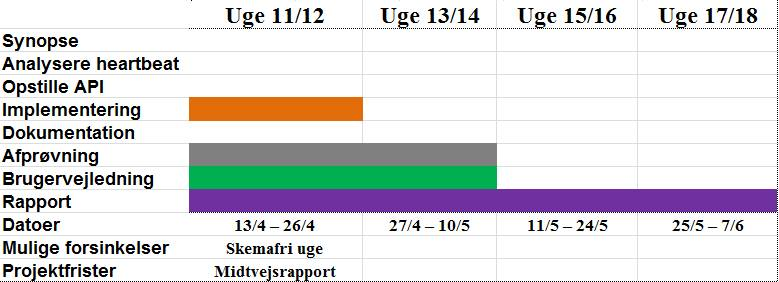
\includegraphics[scale=0.5]{tidsplanmidtvej.jpg}




\section*{Litteraturhenvisninger}


\end{document}
